\documentclass[pdfpagelabels=false, usepdftitle=false, aspectratio=169,10pt]{beamer}
\usetheme[navigation, sectiontitles]{UM}


% ----------------------
% title page information
% ----------------------

\title[Outline]{Exercice sessions}
\subtitle{LDATS2350}

\author[Me]{
  Guillaume Deside \inst{1}
}

\institute[UM]{
  \inst{1} ISBA, Institut de Statistique, Biostatistique et Sciences Actuarielles \\
}

\date{\today}


% ---------------------
% begin of presentation
% ---------------------

\begin{document}


\UMtitleframe  % note that we *do not* use \titlepage


% ----Frame------------

\begin{frame}{Outline}
    {\small \tableofcontents}
\end{frame}


% ----Frame------------

%\section{Pratical informations}
% Slide: Tutor Information
\begin{frame}[fragile]{Tutor Information}
\begin{description}
  \item[Name:] Guillaume Deside
  \item[Office:] Office D374, Voie du Roman Pays 20 (ISBA)
  \item[Office Hours:] By appointment
  \item[Contact:] \texttt{guillaume.deside@uclouvain.be}
\end{description}
\end{frame}

\begin{frame}[fragile]{Coursebook Objectives and Usage}
\textbf{The objective of this coursebook} is to put into practice the concepts and theory 
seen during the theoretical lectures. The main part of the exercises will involve using 
\textbf{SAS Viya}. Still, some exercises and examples are to be solved by hand or may 
require a bit of coding in \textbf{R}.

\vspace{0.3cm}
The difficulty level of the proposed exercises may vary greatly. The goal is to provide challenges for the most motivated students and help them deepen their knowledge through practice.
\end{frame}

% Slide: Overview of the 5 Practical Sessions
\begin{frame}[fragile]{Practical Sessions}
\begin{itemize}
    \item \textbf{Session 1} -- Introduction and Exploring data
    \begin{itemize}
      \item Date: February 10th and 11th
    \end{itemize}
    \vfill
    \item \textbf{Session 2} -- Exploring data and Regression model
    \begin{itemize}
      \item Date: February 24th and 25th
    \end{itemize}
    \vfill
    \item \textbf{Session 3} -- Models
    \begin{itemize}
      \item Date: March 11th and 17th
    \end{itemize}
    \vfill
    \item \textbf{Session 4} -- End exercises 
    \begin{itemize}
      \item Date: March 24th and 25th
    \end{itemize}
    \vfill
    \item \textbf{Session 5} -- Questions/answes
    \begin{itemize}
      \item Date: April 7th and 8th
    \end{itemize}
\end{itemize}
\end{frame}

\begin{frame}{Course Overview - Practical Sessions}
\textbf{TP1: Introduction to SAS Enterprise Miner, Accessing and Preparing Data, Exploratory Analysis}
\begin{itemize}
    \item Introduction
    \item Creating a project
    \item Exploring data (histogram, plots, exploring variable associations)
    \item The Curse of Dimensionality
\end{itemize}

\vspace{0.5cm}
\textbf{TP2: Data Treatment, Partitioning Data, Missing Values, Regressions}
\begin{itemize}
    \item Data treatment (transform variables, variable selection)
    \item Regression
\end{itemize}
\end{frame}

\begin{frame}{Course Overview - Practical Sessions (continued)}
\textbf{TP3: Decision Trees, Neural Networks}
\begin{itemize}
    \item Decision Trees
    \item Neural Networks
\end{itemize}

\textbf{TP4: Model Assessment, ROC Charts}
\begin{itemize}
    \item Comparing models with summary statistics
    \item Statistical graphics (ROC chart, cumulative lift, \dots)
\end{itemize}
\end{frame}




% Slide: Additional Practical Information (Example)
\begin{frame}[fragile]{Additional Practical Information}
\begin{enumerate}
  \item \textbf{Bring your own laptop}: Make sure all required software is installed. (If needed, I can provide a computer in exchange for the student card)
  \item \textbf{Check the course Moodle}: Materials and updates will be posted.
\end{enumerate}
\end{frame}





%\section{Exercise session 1}

\subsection{Reminders}
\begin{frame}{Reminding: What is Regression?}
\begin{itemize}
    \item \textbf{Regression} is a family of methods used to model and analyze the relationship between:
    \begin{itemize}
        \item A \textit{dependent variable} (often denoted \(Y\)), and
        \item One or more \textit{independent} (or explanatory) variables (often denoted \(X_1, X_2, \ldots, X_n\)).
    \end{itemize}
    \item The goal is to \textbf{predict} the value of \(Y\) for given new values of the independent variables or to understand how \(Y\) changes when any one of the \(X_j\) changes.
    \item Many types of regression models exist (linear, polynomial, logistic, etc.), each making different assumptions about how the variables are related.
\end{itemize}
\end{frame}


\begin{frame}{Linear Regression: Definition}
\textbf{Linear Regression} models the \textit{expected value} of \(Y\) as a \textbf{linear} combination of the input variables \(X_1, X_2, \dots, X_n\).

\begin{block}{General Form}
\[
Y = \underbrace{w_1 X_1 + w_2 X_2 + \cdots + w_n X_n}_{\text{linear combination}} + b
\]
\[
= \sum_{j=1}^{n} w_j X_j + b,
\]
where:
\begin{itemize}
    \item \(w_j\) (for \(j = 1, \dots, n\)) are \textbf{weights} (or coefficients).
    \item \(b\) is the \textbf{intercept} (also called bias in some contexts).
\end{itemize}
\end{block}
\end{frame}

%------------------------------------------------------------
% Slide: Simple Linear Regression
%------------------------------------------------------------
\begin{frame}{Simple Linear Regression (\(n=1\))}
\begin{itemize}
    \item When there is only \(\mathbf{1}\) independent variable, \(X = X_1\), the model is called \textbf{simple linear regression}.
    \item The model then reduces to:
    \[
    Y = w\,X + b.
    \]
    \item \textbf{Interpretation}:
    \begin{itemize}
        \item \(w\) measures the change in \(Y\) associated with a one-unit change in \(X\).
        \item \(b\) is the value of \(Y\) when \(X=0\).
    \end{itemize}
\end{itemize}
\end{frame}

%------------------------------------------------------------
% Slide: Advantages and Assumptions of Linear Regression
%------------------------------------------------------------
\begin{frame}{Advantages \& Assumptions of Linear Regression}
\textbf{Advantages:}
\begin{itemize}
    \item Simple and \textbf{easy to interpret}.
    \item Works well if the \textbf{linear assumption} is reasonably accurate.
    \item Efficient to \textbf{train} (closed-form solutions or rapid iterative methods exist).
\end{itemize}

\vfill

\textbf{Common Assumptions:}
\begin{itemize}
    \item \textbf{Linearity:} \(Y\) is linearly related to \(X_1, \dots, X_n\).
    \item \textbf{Independence:} Observations are independently sampled.
    \item \textbf{Homoscedasticity:} Constant variance of errors across the range of predictor variables.
    \item \textbf{Normality of Errors (optional in some contexts):} Residuals (errors) are normally distributed.
\end{itemize}
\end{frame}


\begin{frame}{Introduction to Classification Metrics}
    \begin{itemize}
        \item Metrics used to evaluate the performance of classification models.
        \item Common metrics: Accuracy, Precision, Recall, F1 Score.
    \end{itemize}
\end{frame}

\begin{frame}{Confusion Matrix}
    \begin{itemize}
        \item Table used to describe the performance of a classification model.
        \item Components: True Positives (TP), True Negatives (TN), False Positives (FP), False Negatives (FN).
    \end{itemize}

    \begin{table}[h!]
    \centering
    \begin{tabular}{|c|c|c|}
        \hline
        & \textbf{Predicted: FALSE} & \textbf{Predicted: TRUE} \\
        \hline
        \textbf{Actual: FALSE} & True Negative (TN) & False Positive (FP) \\
        \hline
        \textbf{Actual: TRUE} & False Negative (FN) & True Positive (TP) \\
        \hline
    \end{tabular}
    \caption{Confusion Matrix}
    \label{tab:confusion_matrix}
\end{table}
\end{frame}


\begin{frame}{Accuracy}
    \begin{itemize}
        \item Ratio of correctly predicted instances to the total instances.
        \item Formula:
        \[
        \text{Accuracy} = \frac{TP + TN}{TP + TN + FP + FN}
        \]
        \item Suitable when classes are balanced.
    \end{itemize}
\end{frame}

\begin{frame}{Precision}
    \begin{itemize}
        \item Ratio of correctly predicted positive observations to the total predicted positives.
        \item Formula:
        \[
        \text{Precision} = \frac{TP}{TP + FP}
        \]
        \item Focuses on the correctness of positive predictions.
    \end{itemize}
\end{frame}

\begin{frame}{Recall (Sensitivity)}
    \begin{itemize}
        \item Ratio of correctly predicted positive observations to all observations in the actual class.
        \item Formula:
        \[
        \text{Recall} = \frac{TP}{TP + FN}
        \]
        \item Measures the ability to identify all relevant instances.
    \end{itemize}
\end{frame}

\begin{frame}{F1 Score}
    \begin{itemize}
        \item Harmonic mean of Precision and Recall.
        \item Formula:
        \[
        F1 \text{ Score} = 2 \times \frac{\text{Precision} \times \text{Recall}}{\text{Precision} + \text{Recall}}
        \]
        \item Useful when you need a balance between Precision and Recall.
    \end{itemize}
\end{frame}


\begin{frame}{ROC-AUC Curve}
    \begin{itemize}
        \item Receiver Operating Characteristic - Area Under Curve.
        \item Plots True Positive Rate (TPR) against False Positive Rate (FPR).
        \item Measures the ability of the model to distinguish between classes.
    \end{itemize}
\end{frame}

\begin{frame}{Precision-Recall Curve}
    \begin{itemize}
        \item Plots Precision against Recall.
        \item Useful when dealing with imbalanced datasets.
        \item Focuses on the performance of the positive class.
    \end{itemize}
\end{frame}


\input{Sections/TP1/Exercises}

%\section{Exercise session 2}
\subsection{Reminders}
\begin{frame}{Reminding: What is Regression?}
\begin{itemize}
    \item \textbf{Regression} is a family of methods used to model and analyze the relationship between:
    \begin{itemize}
        \item A \textit{dependent variable} (often denoted \(Y\)), and
        \item One or more \textit{independent} (or explanatory) variables (often denoted \(X_1, X_2, \ldots, X_n\)).
    \end{itemize}
    \item The goal is to \textbf{predict} the value of \(Y\) for given new values of the independent variables or to understand how \(Y\) changes when any one of the \(X_j\) changes.
    \item Many types of regression models exist (linear, polynomial, logistic, etc.), each making different assumptions about how the variables are related.
\end{itemize}
\end{frame}


\begin{frame}{Linear Regression: Definition}
\textbf{Linear Regression} models the \textit{expected value} of \(Y\) as a \textbf{linear} combination of the input variables \(X_1, X_2, \dots, X_n\).

\begin{block}{General Form}
\[
Y = \underbrace{w_1 X_1 + w_2 X_2 + \cdots + w_n X_n}_{\text{linear combination}} + b
\]
\[
= \sum_{j=1}^{n} w_j X_j + b,
\]
where:
\begin{itemize}
    \item \(w_j\) (for \(j = 1, \dots, n\)) are \textbf{weights} (or coefficients).
    \item \(b\) is the \textbf{intercept} (also called bias in some contexts).
\end{itemize}
\end{block}
\end{frame}

%------------------------------------------------------------
% Slide: Simple Linear Regression
%------------------------------------------------------------
\begin{frame}{Simple Linear Regression (\(n=1\))}
\begin{itemize}
    \item When there is only \(\mathbf{1}\) independent variable, \(X = X_1\), the model is called \textbf{simple linear regression}.
    \item The model then reduces to:
    \[
    Y = w\,X + b.
    \]
    \item \textbf{Interpretation}:
    \begin{itemize}
        \item \(w\) measures the change in \(Y\) associated with a one-unit change in \(X\).
        \item \(b\) is the value of \(Y\) when \(X=0\).
    \end{itemize}
\end{itemize}
\end{frame}

%------------------------------------------------------------
% Slide: Advantages and Assumptions of Linear Regression
%------------------------------------------------------------
\begin{frame}{Advantages \& Assumptions of Linear Regression}
\textbf{Advantages:}
\begin{itemize}
    \item Simple and \textbf{easy to interpret}.
    \item Works well if the \textbf{linear assumption} is reasonably accurate.
    \item Efficient to \textbf{train} (closed-form solutions or rapid iterative methods exist).
\end{itemize}

\vfill

\textbf{Common Assumptions:}
\begin{itemize}
    \item \textbf{Linearity:} \(Y\) is linearly related to \(X_1, \dots, X_n\).
    \item \textbf{Independence:} Observations are independently sampled.
    \item \textbf{Homoscedasticity:} Constant variance of errors across the range of predictor variables.
    \item \textbf{Normality of Errors (optional in some contexts):} Residuals (errors) are normally distributed.
\end{itemize}
\end{frame}


\begin{frame}{Introduction to Classification Metrics}
    \begin{itemize}
        \item Metrics used to evaluate the performance of classification models.
        \item Common metrics: Accuracy, Precision, Recall, F1 Score.
    \end{itemize}
\end{frame}

\begin{frame}{Confusion Matrix}
    \begin{itemize}
        \item Table used to describe the performance of a classification model.
        \item Components: True Positives (TP), True Negatives (TN), False Positives (FP), False Negatives (FN).
    \end{itemize}

    \begin{table}[h!]
    \centering
    \begin{tabular}{|c|c|c|}
        \hline
        & \textbf{Predicted: FALSE} & \textbf{Predicted: TRUE} \\
        \hline
        \textbf{Actual: FALSE} & True Negative (TN) & False Positive (FP) \\
        \hline
        \textbf{Actual: TRUE} & False Negative (FN) & True Positive (TP) \\
        \hline
    \end{tabular}
    \caption{Confusion Matrix}
    \label{tab:confusion_matrix}
\end{table}
\end{frame}


\begin{frame}{Accuracy}
    \begin{itemize}
        \item Ratio of correctly predicted instances to the total instances.
        \item Formula:
        \[
        \text{Accuracy} = \frac{TP + TN}{TP + TN + FP + FN}
        \]
        \item Suitable when classes are balanced.
    \end{itemize}
\end{frame}

\begin{frame}{Precision}
    \begin{itemize}
        \item Ratio of correctly predicted positive observations to the total predicted positives.
        \item Formula:
        \[
        \text{Precision} = \frac{TP}{TP + FP}
        \]
        \item Focuses on the correctness of positive predictions.
    \end{itemize}
\end{frame}

\begin{frame}{Recall (Sensitivity)}
    \begin{itemize}
        \item Ratio of correctly predicted positive observations to all observations in the actual class.
        \item Formula:
        \[
        \text{Recall} = \frac{TP}{TP + FN}
        \]
        \item Measures the ability to identify all relevant instances.
    \end{itemize}
\end{frame}

\begin{frame}{F1 Score}
    \begin{itemize}
        \item Harmonic mean of Precision and Recall.
        \item Formula:
        \[
        F1 \text{ Score} = 2 \times \frac{\text{Precision} \times \text{Recall}}{\text{Precision} + \text{Recall}}
        \]
        \item Useful when you need a balance between Precision and Recall.
    \end{itemize}
\end{frame}


\begin{frame}{ROC-AUC Curve}
    \begin{itemize}
        \item Receiver Operating Characteristic - Area Under Curve.
        \item Plots True Positive Rate (TPR) against False Positive Rate (FPR).
        \item Measures the ability of the model to distinguish between classes.
    \end{itemize}
\end{frame}

\begin{frame}{Precision-Recall Curve}
    \begin{itemize}
        \item Plots Precision against Recall.
        \item Useful when dealing with imbalanced datasets.
        \item Focuses on the performance of the positive class.
    \end{itemize}
\end{frame}



\section{Exercise session 3}

\subsection{Reminders}

\begin{frame}{\textcolor{darkblue}{What is K-Nearest Neighbors (KNN)?}}
    \textbf{\textcolor{darkred}{K-Nearest Neighbors (KNN)}} is a \textbf{simple yet powerful classification algorithm} used in machine learning.
    \vspace{0.5cm}
    
    It is a \textbf{non-parametric, lazy learning algorithm} that makes predictions based on the similarity between data points.

    \textbf{Key Idea:}
    \begin{itemize}
        \item "A data point is classified based on the majority class of its \textbf{k nearest neighbors}."
        \item Works well for \textbf{pattern recognition, recommendation systems, and anomaly detection}.
    \end{itemize}
\end{frame}

% Slide 2: How KNN Works
\begin{frame}{\textcolor{darkblue}{How Does KNN Work?}}
    \textbf{\textcolor{darkred}{Step-by-Step Process:}}
    \begin{enumerate}
        \item \textbf{Choose a value for \( k \)} (number of neighbors to consider).
        \item  \textbf{Calculate the distance} between the new data point and all other points in the dataset (e.g., \textbf{Euclidean distance}).
        \item  \textbf{Select the \( k \) nearest neighbors} based on the smallest distances.
        \item  \textbf{Assign the most common class} among the neighbors to the new data point.
    \end{enumerate}
\end{frame}

% Slide 3: Illustration of KNN
\begin{frame}{\textcolor{darkblue}{Illustration of KNN}}
    \begin{columns}
        % Left Column - Explanation
        \column{0.5\textwidth}
        \textbf{\textcolor{darkred}{Visual Representation:}}
        \medskip

        \textbf{Explanation:}
        \begin{itemize}
            \item The \textbf{blue and red dots} represent different classes.
            \item The \textbf{green dot} is the new observation we want to classify.
            \item The \textbf{KNN algorithm} looks at its nearest \( k \) neighbors (e.g., \( k=5 \)).
            \item The majority of neighbors belong to the \textbf{blue class}, so the new observation is classified as \textbf{blue}.
        \end{itemize}
        
        % Right Column - Image
        \column{0.5\textwidth}
        \centering
        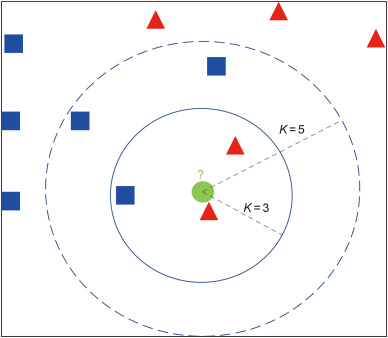
\includegraphics[width=\linewidth]{Sections/TP3/Images/KNN.jpg}
    \end{columns}
\end{frame}


\begin{frame}{\textcolor{darkblue}{What is a Decision Tree?}}
    A \textbf{Decision Tree} is a supervised learning algorithm used for classification and regression tasks.  
    It \textbf{splits} the dataset into smaller subsets based on feature conditions, forming a tree-like structure.
    
    \vspace{0.4cm}
    \textbf{Key Characteristics:}
    \begin{itemize}
        \item Works well for both classification and regression tasks.
        \item Models non-linear relationships
        effectively.
        \item \textbf{Interpretable} and mimics human decision-making.
    \end{itemize}
\end{frame}

% Slide 2: Why Use Decision Trees?
\begin{frame}{\textcolor{darkblue}{Why Use Decision Trees?}}
    \textbf{Advantages:}
    \begin{itemize}
        \item Easy to Understand & Interpret - Mimics human decision-making.
        \item No Need for Feature Scaling - Works with raw data.
        \item Handles Both Numerical & Categorical Data - Highly versatile.
        \item Feature Importance - Identifies significant attributes automatically.
    \end{itemize}
    
    \textbf{Disadvantages:}
    \begin{itemize}
        \item Prone to Overfitting: Deep trees memorize training data.
        \item Sensitive to Noisy Data: Small changes can lead to different trees.
        \item Not Always the Best Model: Ensemble methods like Random Forest may be better.
    \end{itemize}
\end{frame}

% Slide 3: Key Components of a Decision Tree
\begin{frame}{\textcolor{darkblue}{Key Components of a Decision Tree}}
    \textbf{Structure of a Decision Tree:}
    \begin{itemize}
        \item \textbf{Root Node}: The starting point of the tree.
        \item  \textbf{Decision Nodes}: Intermediate nodes that split based on conditions.
        \item \textbf{Leaf Nodes}: Final nodes that provide the classification.
    \end{itemize}

    \textbf{Splitting Criteria:}
    \begin{itemize}
        \item \textbf{Gini Impurity}: Measures impurity in a split.
        \item \textbf{Entropy (Information Gain)}: Measures disorder in the dataset.
    \end{itemize}
\end{frame}

\begin{frame}{\textcolor{darkblue}{How Does a Decision Tree Work?}}
    \textbf{Step-by-Step Process:}
    \begin{enumerate}
        \item \textbf{Find the Best Feature to Split:} Select using \textbf{Gini Impurity} or \textbf{Entropy (Information Gain)}.
        \item \textbf{Recursive Splitting:} Continue partitioning until a stopping criterion is met.
        \item \textbf{Assign Class Labels:} The final \textbf{leaf nodes} contain the class predictions.
    \end{enumerate}
\end{frame}

% Slide 2: Classification Trees - Splitting Overview
\begin{frame}{\textcolor{darkblue}{Classification Trees: Splitting Overview}}
    \textbf{Goal}: Recursively partition the training set into \textit{purer} subsets with respect to the \textbf{target class}.

    \begin{itemize}
        \item \textbf{Node Impurity}: Measures how \emph{mixed} a node is in terms of class distribution.
        \item \textbf{Splitting Criterion}: Common measures of impurity include:
            \begin{itemize}
                \item \textbf{Gini Index}
                \item \textbf{Entropy (Information Gain)}
            \end{itemize}
        \item At each node, the algorithm selects:
            \begin{itemize}
                \item \textbf{Feature} and a \textbf{threshold} (for numeric features)
                \item \textbf{Category partition} (for categorical features)
            \end{itemize}
            that minimizes impurity after the split.
        \item Splitting continues until a stopping criterion is met:
            \begin{itemize}
                \item \textbf{Max depth} reached
                \item \textbf{Minimum samples per leaf} met
                \item \textbf{Minimal impurity reduction} threshold satisfied
            \end{itemize}
    \end{itemize}
\end{frame}

% Slide 3: Gini Index Definition
\begin{frame}{\textcolor{darkblue}{Classification Trees: Gini Index}}
\small
    \textbf{Definition:} The \textbf{Gini Index} at a node with classes \( C_1, C_2, \dots, C_m \) is:
    \[
    \text{Gini}(\text{node}) = \sum_{j=1}^{m} p_j \,(1 - p_j),
    \]
    where \( p_j \) is the \emph{proportion} of samples in the node belonging to class \( C_j \).

    \medskip
    \textbf{Alternative Form:}

    $$\text{Gini}(\text{node}) = 1 - \sum_{j=1}^{m} p_j^2.$$
    
    \textbf{Interpretation:}
    \begin{itemize}
        \item If all samples belong to \emph{one class} (\( p_j = 1 \) for some \( j \)), then \( \text{Gini} = 0 \) (\textit{pure} node).
        \item If classes are \textbf{evenly distributed} (\( p_j = 1/m \)), then \( \text{Gini} \) is \textbf{maximal}, indicating \textit{maximum impurity}.
    \end{itemize}
\end{frame}

% Slide 4: Entropy and Information Gain
\begin{frame}{\textcolor{darkblue}{Classification Trees: Entropy and Information Gain}}
\small
    \textbf{Entropy:} Measures the uncertainty of a dataset before and after splitting.

    \[
    H(\text{node}) = - \sum_{j=1}^{m} p_j \log_2 (p_j)
    \]

    \textbf{Information Gain (IG)}:
    \[
    \text{IG} = H(\text{parent}) - \sum_{i=1}^{k} \frac{|D_i|}{|D|} H(D_i)
    \]

    where:
    \begin{itemize}
        \item \( H(\text{parent}) \) = entropy before the split
        \item \( H(D_i) \) = entropy of subset \( D_i \) after the split
        \item \( |D_i| / |D| \) = proportion of samples in \( D_i \)
    \end{itemize}

    \textbf{Higher Information Gain} means Better feature split.
\end{frame}

% Slide 5: Decision Tree Example
\begin{frame}{\textcolor{darkblue}{Decision Tree Visualization Example}}
    \centering
    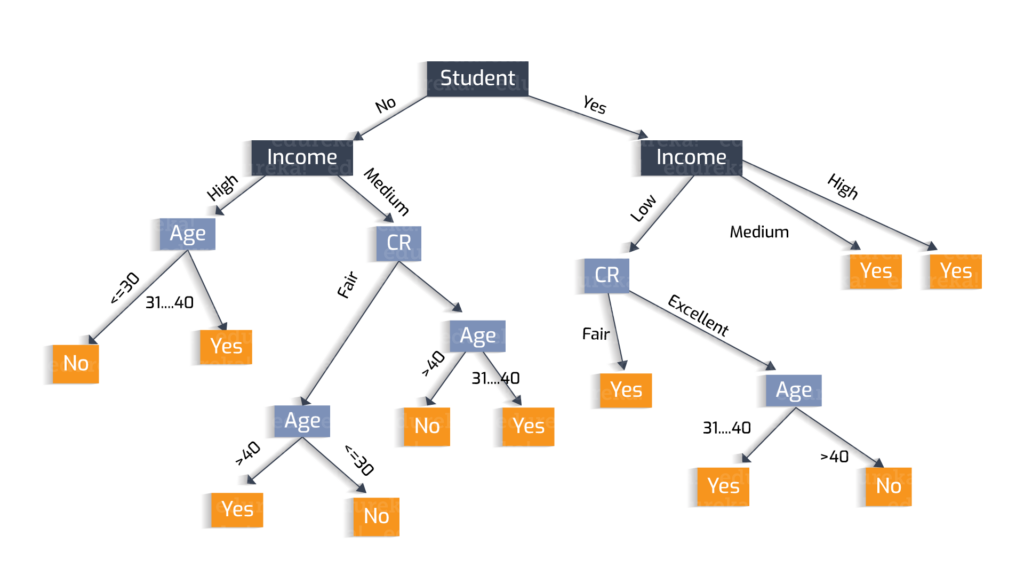
\includegraphics[width=0.75\linewidth]{Sections/TP3/Images/decision_tree.png}

    \medskip
    \textbf{Example:} A decision tree trained.
\end{frame}

% Slide 5: Tuning Hyperparameters
\begin{frame}{\textcolor{darkblue}{Tuning Hyperparameters}}
    You can optimize decision tree performance by adjusting:
    \begin{itemize}
        \item max\_depth : Limits tree depth to prevent overfitting.
        \item min\_samples\_split : Minimum samples needed to split a node.
        \item min\_samples\_leaf : Minimum samples required in a leaf node.
        \item criterion : `"gini"` (default) or `"entropy"` for calculating splits.
    \end{itemize}
\end{frame}

\begin{frame}{\textcolor{darkblue}{What is Naive Bayes?}}
    \textbf{Naive Bayes} is a probabilistic classification algorithm based on \textbf{Bayes' Theorem}.  
    It is widely used for:
    \begin{itemize}
        \item \textbf{Text classification}
        \item \textbf{Spam detection}
        \item \textbf{Sentiment analysis}
        \item \textbf{Medical diagnosis}
    \end{itemize}

    \vspace{0.4cm}
    \textbf{Bayes' Theorem:}
    \[
    P(A|B) = \frac{P(B|A) \cdot P(A)}{P(B)}
    \]
\end{frame}

% Slide 2: Why is it "Naïve"?
\begin{frame}{\textcolor{darkblue}{Why is it "Naive"?}}
    The algorithm is called "naive" because it assumes that \textbf{all features are independent} given the class label.  
    This simplifies computation and works well despite often being unrealistic.
\end{frame}

% Slide 3: Bayes Theorem in Classification
\begin{frame}{\textcolor{darkblue}{Bayes Theorem in Naive Bayes Classification}}
    \textbf{Bayes' Theorem Formula:}
    \[
    p(y|\mathbf{x}) = \frac{p(\mathbf{x}|y)p(y)}{p(\mathbf{x})} = \frac{p(\mathbf{x}|y)p(y)}{\sum_{i=1}^H p(\mathbf{x}|y_i)p(y_i)}
    \]
    where:
    \begin{itemize}
        \item $ p(y|\mathbf{x}) $ - Posterior probability of class $ y $.
        \item $ p(\mathbf{x}|y) $ - Likelihood of feature $ \mathbf{x} $.
        \item $ p(y) $ - Prior probability of class $ y $.
        \item $ p(\mathbf{x}) $ - Normalization factor.
    \end{itemize}
\end{frame}

% Slide 4: Maximum A Posteriori (MAP) Hypothesis
\begin{frame}{\textcolor{darkblue}{Maximum A Posteriori (MAP) Hypothesis}}
    \[
    y_{MAP} = \arg \max_{y \in H} p(\mathbf{x}|y)p(y)
    \]
    We classify a sample by choosing the class that maximizes the product of the likelihood and the prior.
\end{frame}

% Slide 5: Naïve Independence Assumption
\begin{frame}{\textcolor{darkblue}{Naive Independence Assumption}}
    \[
    P(\mathbf{x}|y) = \prod_{j=1}^n P(x_j|y)
    \]
    This simplifies computation since we do not need to compute joint probabilities for multiple features.
\end{frame}

% Slide 6: Handling Categorical & Numerical Data
\begin{frame}{\textcolor{darkblue}{Handling Categorical & Numerical Data}}
    \textbf{Categorical Attributes:}
    \[
    P(x_j|y) = P(x_j = r_{jk} | y = v_n)
    \]
    \textbf{Numerical Attributes (Gaussian Assumption):}
    \[
    P(x_j|y) \sim N(\mu_{jh}, \sigma_{jh}^2)
    \]
\end{frame}

% Slide 7: Advantages & Disadvantages
\begin{frame}{\textcolor{darkblue}{Advantages & Disadvantages}}
    \textbf{Advantages:}
    \begin{itemize}
        \item Fast and scalable.
        \item Handles missing data well.
        \item Works well with text classification.
        \item Easy to interpret.
    \end{itemize}

    \textbf{Disadvantages:}
    \begin{itemize}
        \item Assumes feature independence (which is often unrealistic).
        \item Zero probability issue (if a category never appears in training data).
    \end{itemize}
\end{frame}

\begin{frame}{\textcolor{darkblue}{What is Logistic Regression?}}
    Logistic Regression is a \textbf{supervised learning algorithm} used for \textbf{binary classification} problems.
    
    \textbf{Key Characteristics:}
    \begin{itemize}
        \item Used for \textbf{binary classification} (e.g., Yes/No, Spam/Not Spam).
        \item Outputs a probability score between \textbf{0 and 1}.
        \item Uses the \textbf{sigmoid function} to map real values to probabilities.
        \item The decision boundary is defined by a threshold (e.g., \textbf{0.5}).
    \end{itemize}
\end{frame}

% Slide 2: The Logistic (Sigmoid) Function
\begin{frame}{\textcolor{darkblue}{The Logistic (Sigmoid) Function}}
    The logistic function is defined as:

    \[
    \sigma(z) = \frac{1}{1 + e^{-z}}
    \]

    where:

    \[
    z = w_1 X_1 + w_2 X_2 + ... + w_n X_n + b = \mathbf{w}^T \mathbf{x} + b
    \]

    \begin{itemize}
        \item $X$ = feature vector
        \item $w$ = weight coefficients
        \item $b$ = bias term
        \item $e$ = Euler’s number ($\approx 2.718$)
    \end{itemize}

    \textbf{Decision Rule:}
    \[
    \hat{y} =
    \begin{cases} 
    1, & \text{if } \sigma(z) \geq 0.5 \\ 
    0, & \text{otherwise}
    \end{cases}
    \]
\end{frame}

% Slide 3: Cost Function for Logistic Regression
\begin{frame}{\textcolor{darkblue}{Cost Function for Logistic Regression}}
    Logistic Regression does not use Mean Squared Error (MSE) as its cost function because it leads to a \textbf{non-convex function}, making optimization difficult.

    Instead, we maximize the likelihood:

    \[
    L(w) := \prod_{i=1}^{n} P(Y_i = y_i | w, x_i)
    \]

    Assuming independence:

    \[
    L(w) := \prod_{i|y_i=1} p(x_i) * \prod_{i|y_i=0}(1- p(x_i))
    \]

    \[
    L(w) := \prod_{i=1}^{n} p(x_i)^{y_i}(1- p(x_i))^{1-y_i}
    \]
\end{frame}

\begin{frame}{\textcolor{darkblue}{Cost Function for Logistic Regression}}
    
    The log-likelihood function is:

    \[
    l(w) = \sum_{i=1}^{n} \left( y_i \log(p(x_i)) + (1-y_i) \log(1- p(x_i)) \right)
    \]

    \[
    = \sum_{i=1}^{n} \left( y_i \log\left(\frac{p(x_i)}{1-p(x_i)}\right) + \log(1-p(x_i)) \right)
    \]

    \textbf{Optimization Problem:}
    \[
    \min_{w} \frac{1}{2}||w||^2 + C \sum_{i=1}^{n} \left( y_i w^T x_i - \log(1-e^{w^T x_i}) \right)
    \]
\end{frame}

% Slide 4: Logistic Regression vs Linear Regression
\begin{frame}{\textcolor{darkblue}{Logistic Regression vs Linear Regression}}
    \begin{table}[]
    \small
        \centering
        \begin{tabular}{|c|c|c|}
            \hline
            \textbf{Feature} & \textbf{Linear Regression} & \textbf{Logistic Regression} \\
            \hline
            \textbf{Output Type} & Continuous & Probability (0-1) \\
            \hline
            \textbf{Function Used} & Linear Equation & Sigmoid Function \\
            \hline
            \textbf{Use Case} & Regression & Classification \\
            \hline
            \textbf{Loss Function} & Mean Squared Error (MSE) & Log Loss (Binary Cross Entropy) \\
            \hline
            \textbf{Decision Boundary} & Any real number & Threshold (0.5) \\
            \hline
        \end{tabular}
    \end{table}
\end{frame}

% Slide 5: Visual Representation of Logistic Regression
\begin{frame}{\textcolor{darkblue}{Visual Representation of Logistic Regression}}
    \centering
    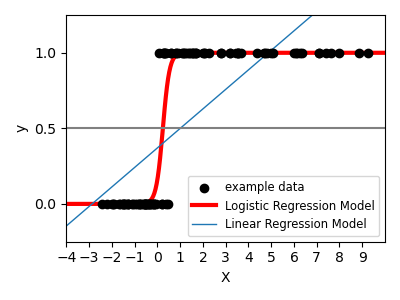
\includegraphics[width=0.7\linewidth]{Sections/TP3/Images/logistic_regression.png}
\end{frame}


\begin{frame}{\textcolor{darkblue}{What is a Support Vector Machine (SVM)?}}
    Support Vector Machine (SVM) is a \textbf{supervised learning algorithm} used for classification and regression tasks.

    \vspace{0.3cm}
    \textbf{Key Features:}
    \begin{itemize}
        \item Works well in \textbf{high-dimensional spaces}.
        \item Finds the \textbf{optimal decision boundary} (hyperplane).
        \item Effective for \textbf{small datasets}.
        \item Uses \textbf{kernel functions} to handle non-linear data.
    \end{itemize}
\end{frame}

% Slide 2: Mathematical Formulation
\begin{frame}{\textcolor{darkblue}{Mathematical Formulation of SVM}}
    The goal of SVM is to find the optimal \textbf{hyperplane} that maximizes the margin while minimizing classification error.

    \textbf{Hyperplane Equation:}
    \[
    w \cdot x + b = 0
    \]
    
    where:
    \begin{itemize}
        \item $w$ is the \textbf{weight vector} (normal to the hyperplane).
        \item $x$ is the \textbf{feature vector}.
        \item $b$ is the \textbf{bias term}.
    \end{itemize}
\end{frame}

% Slide 3: Hard Margin SVM
\begin{frame}{\textcolor{darkblue}{Hard Margin SVM (Linearly Separable Data)}}
    For a dataset with two classes labeled as $ y_i \in \{-1,1\} $, we define the constraints:

    \[
    y_i (w \cdot x_i + b) \geq 1, \quad \forall i
    \]

    The objective function to maximize the margin:

    \[
    \min_{w} \frac{1}{2} ||w||^2
    \]

    \textbf{Condition:} The data must be perfectly separable.
\end{frame}

% Slide 4: Soft Margin SVM
\begin{frame}{\textcolor{darkblue}{Soft Margin SVM (Non-Separable Data)}}
    In real-world datasets, perfect separation is not possible. We introduce \textbf{slack variables} ($\xi_i$):

    \[
    y_i (w \cdot x_i + b) \geq 1 - \xi_i, \quad \forall i
    \]

    The new objective function:

    \[
    \min_{w,b,\xi} \frac{1}{2} ||w||^2 + C \sum_{i=1}^{n} \xi_i
    \]

    where:
    \begin{itemize}
        \item $C$ is the \textbf{regularization parameter}.
        \item It controls the trade-off between maximizing margin and minimizing classification errors.
    \end{itemize}
\end{frame}

% Slide 5: Kernel Trick
\begin{frame}{\textcolor{darkblue}{Kernel Trick for Non-Linear Data}}
    SVM can be extended to non-linearly separable data using the \textbf{kernel trick}.

    Instead of working in the original feature space, we map data to a higher-dimensional space where it becomes linearly separable.

    \vspace{0.3cm}
    \textbf{Common Kernels:}
    \begin{itemize}
        \item \textbf{Linear Kernel:} \quad $K(x_i, x_j) = x_i \cdot x_j$
        \item \textbf{Polynomial Kernel:} \quad $K(x_i, x_j) = (x_i \cdot x_j + c)^d$
        \item \textbf{Radial Basis Function (RBF):}
        \[
        K(x_i, x_j) = \exp\left(-\gamma ||x_i - x_j||^2\right)
        \]
        \item \textbf{Sigmoid Kernel:} \quad $K(x_i, x_j) = \tanh(\alpha x_i \cdot x_j + c)$
    \end{itemize}

\end{frame}


% Slide 6: Advantages and Disadvantages
\begin{frame}{\textcolor{darkblue}{Advantages and Disadvantages of SVM}}
    \textbf{Advantages:}
    \begin{itemize}
        \item Works well in \textbf{high-dimensional spaces}.
        \item \textbf{Effective for small datasets}.
        \item Can model \textbf{non-linear relationships} using kernels.
        \item \textbf{Robust to overfitting}, especially with proper parameter tuning.
    \end{itemize}

    \vspace{0.4cm}
    \textbf{Disadvantages:}
    \begin{itemize}
        \item Computationally \textbf{expensive} for large datasets.
        \item \textbf{Difficult to interpret} compared to decision trees.
        \item Choice of \textbf{kernel and hyperparameters} requires careful tuning.
    \end{itemize}
\end{frame}

% Slide 7: Visualizing SVM Kernels
\begin{frame}{\textcolor{darkblue}{Visualizing SVM with Different Kernels}}
\centering
    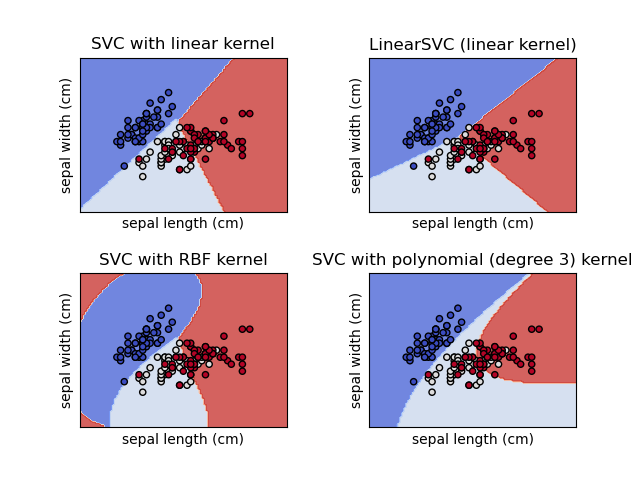
\includegraphics[width=0.65\linewidth]{Sections/TP3/Images/SVM_kernel.png}
\end{frame}


\begin{frame}{\textcolor{darkblue}{What is a Multi-Layer Perceptron (MLP)?}}
    A \textbf{Multi-Layer Perceptron (MLP)} is a type of artificial neural network (ANN) that consists of \textbf{multiple layers} of neurons.

    \vspace{0.3cm}
    \textbf{Key Features:}
    \begin{itemize}
        \item Can model \textbf{non-linear relationships}.
        \item Uses \textbf{backpropagation} for learning.
        \item Suitable for \textbf{classification and regression}.
        \item Works well with \textbf{structured and unstructured data}.
    \end{itemize}
\end{frame}

% Slide 2: Structure of an MLP
\begin{frame}{\textcolor{darkblue}{Structure of an MLP}}
    An MLP consists of the following layers:

    \begin{enumerate}
        \item \textbf{Input Layer} - Receives raw input features.
        \item \textbf{Hidden Layers} - Extracts meaningful patterns using activation functions.
        \item \textbf{Output Layer} - Produces final predictions (softmax for classification, linear for regression).
    \end{enumerate}

    \centering
    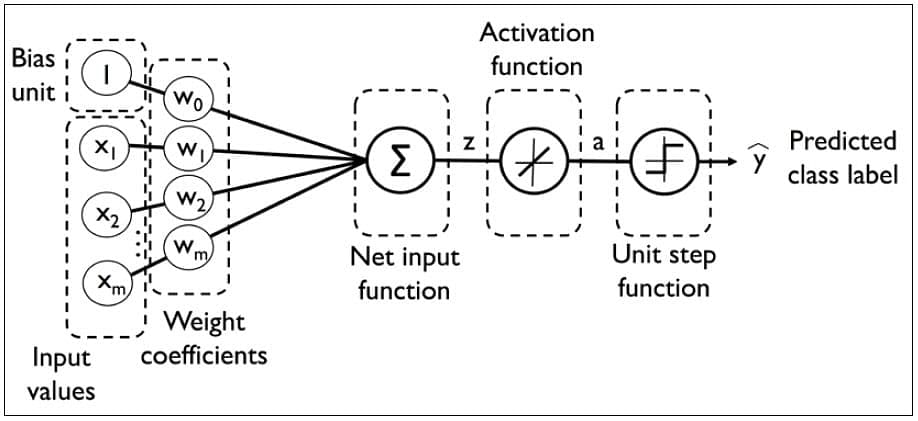
\includegraphics[width=0.6\linewidth]{Sections/TP3/Images/MLP.jpg}
\end{frame}

% Slide 3: Forward Propagation
\begin{frame}{\textcolor{darkblue}{MLP Forward Propagation}}
    Each neuron applies a transformation:

    \[
    z = W \cdot X + b
    \]

    where:
    \begin{itemize}
        \item $ W $ = Weights
        \item $ X $ = Input features
        \item $ b $ = Bias
    \end{itemize}

    Then, an \textbf{activation function} is applied:

    \[
    a = f(z)
    \]

    where $ f(x) $ can be:
    \begin{itemize}
        \item \textbf{ReLU}: $ f(x) = \max(0, x) $
        \item \textbf{Sigmoid}: $ f(x) = \frac{1}{1+e^{-x}} $ (for binary classification)
        \item \textbf{Softmax}: Converts scores into probabilities (for multi-class classification)
    \end{itemize}
\end{frame}


% Slide 5: Applications of MLP
\begin{frame}{\textcolor{darkblue}{Applications of MLP}}
    \begin{itemize}
        \item \textbf{Image Recognition} - Object detection and face recognition.
        \item \textbf{Spam Detection} - Classifying emails as spam or non-spam.
        \item \textbf{Medical Diagnosis} - Predicting diseases based on symptoms.
        \item \textbf{Fraud Detection} - Identifying fraudulent transactions.
        \item \textbf{Stock Market Prediction} - Forecasting stock prices.
    \end{itemize}
\end{frame}


% Slide 1: What are Ensemble Methods?
\begin{frame}{\textcolor{darkblue}{What are Ensemble Methods?}}
    \textbf{Ensemble methods} are machine learning techniques that combine multiple models to improve predictive performance.

    \vspace{0.3cm}
    \textbf{Why use ensemble methods?}
    \begin{itemize}
        \item \textbf{Reduce overfitting} - Combines weak models to prevent over-learning.
        \item \textbf{Increase robustness} - More stable predictions.
        \item \textbf{Improve accuracy} - Aggregation leads to better results.
    \end{itemize}

    \vspace{0.3cm}
    Two popular ensemble techniques are:
    \begin{itemize}
        \item \textbf{Random Forest} (Bagging)
        \item \textbf{AdaBoost} (Boosting)
    \end{itemize}
\end{frame}

% Slide 2: What is Random Forest?
\begin{frame}{\textcolor{darkblue}{Random Forest (Bagging)}}
    \textbf{Random Forest} is an ensemble learning method that builds multiple \textbf{decision trees} and combines their predictions to improve accuracy.

    \vspace{0.3cm}
    \textbf{How Random Forest Works:}
    \begin{enumerate}
        \item \textbf{Bootstrapping:} Creates multiple random subsets of the dataset.
        \item \textbf{Train Decision Trees:} Each tree is trained on a different subset.
        \item \textbf{Aggregation:} Uses \textbf{majority voting} (classification) or \textbf{averaging} (regression).
    \end{enumerate}

    \vspace{0.3cm}
    \textbf{Advantages:}
    \begin{itemize}
        \item Handles large datasets well.
        \item Works with both categorical and numerical data.
        \item Less prone to overfitting than individual decision trees.
        \item Reduces variance by combining multiple models.
    \end{itemize}
\end{frame}

% Slide 3: What is AdaBoost?
\begin{frame}{\textcolor{darkblue}{AdaBoost (Boosting)}}
    \textbf{AdaBoost (Adaptive Boosting)} is a boosting algorithm that trains weak classifiers sequentially, giving more focus to incorrectly classified samples.

    \vspace{0.3cm}
    \textbf{How AdaBoost Works:}
    \begin{enumerate}
        \item \textbf{Assign Equal Weights:} Each sample starts with the same weight.
        \item \textbf{Train Weak Learner:} Usually a simple decision tree (stump).
        \item \textbf{Update Weights:} Misclassified points get \textbf{higher} weights.
        \item \textbf{Combine Weak Learners:} Final prediction is a \textbf{weighted sum} of all weak models.
    \end{enumerate}

    \vspace{0.3cm}
    \textbf{Advantages:}
    \begin{itemize}
        \item Can boost weak models into strong models.
        \item Less prone to overfitting than a single decision tree.
    \end{itemize}
\end{frame}

% Slide 4: Random Forest vs AdaBoost
\begin{frame}{\textcolor{darkblue}{Comparison: Random Forest vs. AdaBoost}}
   %\centering
    \begin{tabular}{|l|c|c|}
        \hline
        \textbf{Feature} & \textbf{Random Forest} & \textbf{AdaBoost} \\
        \hline
        \textbf{Base Learner} & Multiple decision trees & Weak learners (e.g., decision stumps) \\
        \hline
        \textbf{Focus} & Reduces variance (bagging) & Reduces bias (boosting) \\
        \hline
        \textbf{Handling Noise} & Works well with noisy data & Sensitive to noise \\
        \hline
        \textbf{Training Speed} & Faster (parallel trees) & Slower (sequential training) \\
        \hline
        \textbf{Overfitting} & Less prone to overfitting & Can overfit on noisy datasets \\
        \hline
    \end{tabular}
\end{frame}

% Slide 5: When to Use Random Forest or AdaBoost?
\begin{frame}{\textcolor{darkblue}{When to Use Random Forest vs. AdaBoost?}}
    \textbf{Use Random Forest if:}
    \begin{itemize}
        \item You have a large dataset with mixed features.
        \item Overfitting is a concern.
        \item You want a faster model with easy tuning.
    \end{itemize}

    \vspace{0.3cm}
    \textbf{Use AdaBoost if:}
    \begin{itemize}
        \item You have clean and well-prepared data.
        \item You need high accuracy with fewer features.
        \item You want to improve weak classifiers (e.g., decision stumps).
    \end{itemize}
\end{frame}


\begin{frame}{\textcolor{darkblue}{Steps in a Classification Data Mining Project}}

        \begin{enumerate}
            \item \textbf{Problem Definition}  
            \small Define the objective and identify the target variable.  

            \item \textbf{Data Collection \& Preprocessing}  
            \small Gather relevant data, handle missing values, and encode categorical variables.  

            \item \textbf{Exploratory Data Analysis (EDA)}  
            \small Visualize and understand data distributions, correlations, and class imbalances.  

            \item \textbf{Feature Engineering}  
            \small Select important features, create new ones, and standardize/normalize data.  

            \item \textbf{Model Selection}  
            \small Choose algorithms such as Decision Trees, Naïve Bayes, SVM, or Neural Networks.  

            \item \textbf{Model Training \& Evaluation}  
            \small Train models, optimize hyperparameters, and validate using cross-validation.  

            \item \textbf{Performance Metrics}  
            \small Use accuracy, precision, recall, F1-score, and ROC curves to evaluate performance.  

        \end{enumerate}


\end{frame}








\input{Sections/TP3/Exercises}





%------------------------------------------------------------
% SLIDE 3: SPLITTING WITH GINI INDEX
%------------------------------------------------------------
\begin{frame}{Classification Trees: Splitting Using Gini Index}
\textbf{Procedure to choose a split}:
\begin{enumerate}
  \item \textbf{Consider a potential split} on feature \(X\) into two child nodes: 
    \[
      \text{Left node: } \{samples \mid X \le t\}, \quad
      \text{Right node: } \{samples \mid X > t\}.
    \]
  \item \textbf{Compute Gini for each child node}:
    \[
      \text{Gini}_L, \quad \text{Gini}_R.
    \]
  \item \textbf{Weighted Gini after split}: 
    \[
      \text{Gini}_{\text{split}} 
      = \frac{n_L}{n}\,\text{Gini}_L + \frac{n_R}{n}\,\text{Gini}_R,
    \]
    where \(n_L\) and \(n_R\) are sample counts in left and right nodes, \(n = n_L + n_R\).
  \item \textbf{Gini Gain (or reduction)}:
    \[
      \Delta \text{Gini}
      = \text{Gini}_{\text{parent}} - \text{Gini}_{\text{split}}.
    \]
    We pick the feature + threshold that \emph{maximizes} this gain.
\end{enumerate}

\textbf{Note}: 
\begin{itemize}
   \item Similar logic applies for multiple branches or categorical features.
   \item If \(\Delta \text{Gini}\) is small, the split is not very informative.
\end{itemize}
\end{frame}






\section{Exercise session 4}
\subsection{Reminders}



\section{Exercise session 5}
\subsection{Reminders}











% ----Ref Frame--------

%\begin{frame}{Bibliography}
%\tiny 
%\bibliographystyle{apalike}
%\bibliography{ref.bib}
%\end{frame}


\end{document}
